\section{Hopr architecture}
\label{appendix:architecture}

\begin{figure}[H]
    \centering
    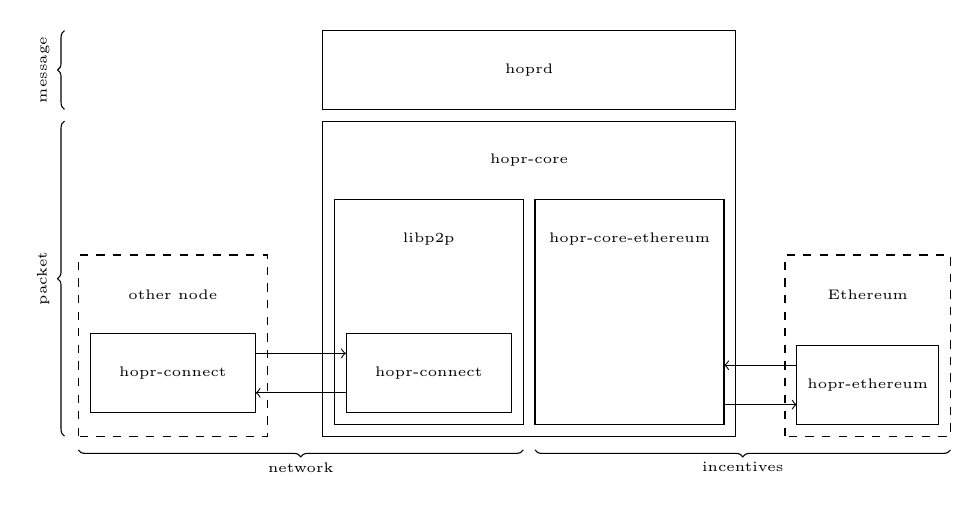
\begin{tikzpicture}
        \def\innersep{0.5}
        \def\coreHeight{4}
        \def\coreWidth{5.25}
        \def\coreEthereumHeight{5}
        \def\coreEthereumWidth{0.5*\coreWidth}
        \def\connectHeight{1}
        \def\connectWidth{\libWidth-3.5*\padding}
        \def\libHeight{3}
        \def\libWidth{0.5*\coreWidth}

        \def\ethereumWidth{2.1}

        \def\otherNodeOffset{3.25}

        \def\ethereumOffset{14}
        \def\padding{0.15}

        % Core
        \draw (0,0) rectangle (\coreWidth,\coreHeight);
        \path (0,\coreHeight-\connectHeight) -- (\coreWidth,\coreHeight) node[midway] {\tiny{hopr-core}};

        % hoprd
        \begin{scope}[shift={(0,\coreHeight+\padding)}]
            \draw (0,0) rectangle (\coreWidth,\connectHeight) node[midway] {\tiny{hoprd}};
        \end{scope}

        % Libp2p
        \path (\padding,\libHeight-\connectHeight) -- (\libWidth-0.5*\padding,\libHeight) node[midway] {\tiny{libp2p}};
        \draw (\padding,\padding) rectangle (\libWidth-0.5*\padding,\libHeight);

        % Core-Ethereum
        \begin{scope}[shift={(0.5*\coreWidth,0)}]
            \path (0.5*\padding,\libHeight-\connectHeight) -- (\libWidth-\padding,\libHeight) node[midway] {\tiny{hopr-core-ethereum}};
            \draw  (0.5*\padding,\padding) rectangle (\coreEthereumWidth-\padding,\libHeight);

        \end{scope}

        % Connect
        \draw[shift={(2*\padding,2*\padding)}] (0,0) rectangle (\connectWidth,\connectHeight) node[midway] {\tiny{hopr-connect}};

        % Connect node 2
        \begin{scope}[shift={(-\otherNodeOffset,0)}]
            \draw[dashed] (\padding,0) rectangle (\connectWidth+3*\padding,2*\connectHeight+2*\padding);
            \path (\padding,\connectHeight+2*\padding) rectangle (\connectWidth+3*\padding,2*\connectHeight+2*\padding) node[midway] {\tiny{other node}};

            \draw[shift={(2*\padding,2*\padding)}] (0,0) rectangle (\connectWidth,\connectHeight) node[midway] {\tiny{hopr-connect}};
        \end{scope}

        % Ethereum
        \begin{scope}[shift={(0.5*\coreWidth+\otherNodeOffset,0)}]
            \draw[dashed] (0,0) rectangle (\ethereumWidth,2*\connectHeight+2*\padding);
            \path (0,\connectHeight+2*\padding) rectangle (\connectWidth,2*\connectHeight+2*\padding) node[midway] {\tiny{Ethereum}};
            \draw (\padding,\padding) rectangle (\ethereumWidth-\padding,\connectHeight+\padding) node[midway] {\tiny{hopr-ethereum}};
        \end{scope}

        % packet <-> message
        \begin{scope}[shift={(-\otherNodeOffset+1*\padding,0)}]
            \draw[decoration={brace,raise=5pt},decorate] (0,0) -- (0,\coreHeight) node[midway,left=7pt] {\rotatebox{90}{\tiny{packet}}};
            \draw[decoration={brace,raise=5pt},decorate] (0,\coreHeight+\padding) -- (0,\coreHeight+\padding+\connectHeight) node[midway,left=7pt] {\rotatebox{90}{\tiny{message}}};
        \end{scope}

        % network <-> incentives
        \draw[decoration={brace,raise=5pt,mirror},decorate] (-\otherNodeOffset+1*\padding,0) -- (\coreWidth*0.5-\padding*0.5,0) node[midway,below=6pt] {\tiny{network}};
        \draw[decoration={brace,raise=5pt,mirror},decorate] (\coreWidth*0.5+\padding*0.5,0) -- (0.5*\coreWidth+\otherNodeOffset+\ethereumWidth,0) node[midway,below=6pt] {\tiny{incentives}};

        % hopr-connect traffic
        \draw[->] (2*\padding,2*\padding+0.25*\connectHeight) -- (-\otherNodeOffset+\connectWidth+2*\padding,2*\padding+0.25*\connectHeight);
        \draw[->] (-\otherNodeOffset+\connectWidth+2*\padding,2*\padding+0.75*\connectHeight) -- (2*\padding,2*\padding+0.75*\connectHeight);

        % smart contract interaction
        \draw[->] (\coreWidth-\padding,1*\padding+0.25*\connectHeight) -- (0.5*\coreWidth+\otherNodeOffset+\padding,\padding+0.25*\connectHeight);
        \draw[->] (0.5*\coreWidth+\otherNodeOffset+\padding,\padding+0.75*\connectHeight) -- (\coreWidth-\padding,\padding+0.75*\connectHeight);
    \end{tikzpicture}
    \caption{Architecture of a HOPR client}
    \label{fig:hoprarchitecture}
\end{figure}
